\appendix

\chapter{Google's Query Expansion Patents}
\label{appendix:googlepatent}
\begin{figure}[h]
    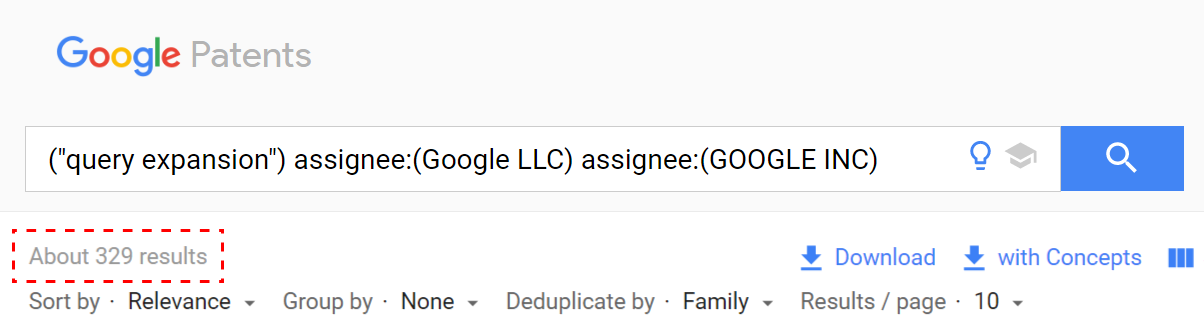
\includegraphics[width=\textwidth]{graphics/google-patents.png}
    \caption{About 329 patents referencing ``query expansion'' owned by Google Inc}
\end{figure}

\begin{table}[h]
\begin{tabular}{ll}
US-9002869-B2    & Machine translation for query expansion                                                                         \\
US-8521761-B2    & Transliteration for query expansion                                                                             \\
US-9146967-B2    & Multi-stage query processing system and method for use with...                               \\
US-9165033-B1    & Efficient query rewriting                                                                                       \\
US-9053115-B1    & Query image search                                                                                              \\
US-8135619-B2    & \textbf{Increasing a number of relevant advertisements using a...}                                            \\
US-9619565-B1    & Generating content snippets using a tokenspace repository                                                       \\
US-9323806-B2    & Clustering query refinements by inferred user intent                                                            \\
US-8600975-B1    & Query phrasification                                                                                            \\
US-8255949-B1    & \textbf{Television program targeting for advertising}                                                                    \\
CN-102349087-B   & Automatically providing content associated with captured information... \\
CN-101796480-B   & Integrating external related phrase information into a phrase-based...       \\
US-8612427-B2    & Information retrieval system for archiving multiple document versions                                           \\
US-9037573-B2    & Phase-based personalization of searches in an information retrieval...                                      \\
\end{tabular}
\end{table}
\begin{table}[]
\begin{tabular}{ll}
US-7617205-B2    & Estimating confidence for query revision models                                                                 \\
US-7870147-B2    & Query revision using known highly-ranked queries                                                                \\
US-7636714-B1    & Determining query term synonyms within query context                                                            \\
US-7565345-B2    & Integration of multiple query revision models                                                                   \\
US-7346615-B2    & Using match confidence to adjust a performance threshold                                                        \\
US-8738553-B1    & Image selection based on image quality                                                                          \\
US-9652483-B1    & Index server architecture using tiered and sharded phrase posting lists                                         \\
US-9183226-B2    & Image classification                                                                                            \\
US-9355169-B1    & Phrase extraction using subphrase scoring                                                                       \\
CN-102226901-B   & Phrase-based searching in an information retrieval system                                                       \\
CN-101133388-B   & Multiple index based information retrieval system                                                               \\
US-7426507-B1    & Automatic taxonomy generation in search results using phrases                                                   \\
US-7580929-B2    & Phrase-based personalization of searches in an information retrieval...                                     \\
US-8996527-B1    & Clustering images                                                                                               \\
US-7702614-B1    & Index updating using segment swapping                                                                           \\
CN-101313300-B   & Local search                                                                                                    \\
US-8825571-B1    & Multiple correlation measures for measuring query similarity                                                    \\
US-2005149499-A1 & Systems and methods for improving search quality                                                                \\
US-9251206-B2    & Generalized edit distance for queries                                                                           \\
US-7925655-B1    & Query scheduling using hierarchical tiers of index servers                                                      \\
US-8452763-B1    & Extracting and scoring class-instance pairs                                                                     \\
US-8832132-B1    & Personalizing search queries based on user membership in social...                             \\
US-9047622-B1    & Delivering content to users based on advertisement interaction type                                             \\
JP-2006048683-A  & Phrase identification method in information retrieval system                                                    \\
JP-2006048685-A  & Indexing method based on phrase in information retrieval system                                                 \\
JP-2006048686-A  & Generation method for document explanation based on phrase                                                      \\
CN-108139849-A   & For the action suggestion of user in selecting content                                                          \\
US-9916396-B2    & Methods and systems for content-based search                                                                    \\
US-9195741-B2    & Triggering music answer boxes relevant to user search queries                                                   \\
US-9507826-B1    & Generating real-time search results                                                                             \\
US-8086594-B1    & Bifurcated document relevance scoring                                                                           \\
KR-20160010652-A & Identifying inadequate search content                                                                           \\
US-10169751-B2   & System and method for point of sale transaction logging                                                         \\
US-2008270364-A1 & Expansion rule evaluation                                                                                       \\
US-8995716-B1    & Image search results by seasonal time period                                                                    \\
\end{tabular}
\end{table}
\begin{table}[]
\begin{tabular}{ll}
CN-107092615-A   & Query suggestion from document                                                                                  \\
US-9767169-B1    & Enhancing search results for improved readability                                                               \\
US-8463783-B1    & Advertisement selection data clustering                                                                         \\
US-8898148-B1    & Targeting to physical environment                                                                               \\
US-8515731-B1    & Synonym verification                                                                                            \\
US-2006230005-A1 & Empirical validation of suggested alternative queries                                                           \\
US-9514223-B1    & Synonym identification based on categorical contexts                                                            \\
US-2015370833-A1 & Visual refinements in image search                                                                              \\
US-8832096-B1    & Query-dependent image similarity                                                                                \\
US-2013018723-A1 & Search-aware conditional bidding on advertisement display                                                       \\
CN-105706135-A   & Supporting voting-based campaigns in search                                                                     \\
US-9218369-B2    & Ranking image search results using hover data                                                                   \\
US-9270712-B2    & Managing moderation of user-contributed edits                                                                   \\
US-8909625-B1    & Image search                                                                                                    \\
US-8538979-B1    & Generating phrase candidates from text string entries                                                           \\
US-9286405-B2    & Index-side synonym generation                                                                                   \\
US-8027938-B1    & Discriminative training in machine learning                                                                     \\
EP-2073131-A1    & Method and apparatus for processing a search query for text content...                                       \\
CN-108463816-A   & Prevent from forbidding the distribution of Web content by using...                    \\
US-9286395-B1    & Modifying query in discourse context                                                                            \\
US-2016307000-A1 & Index-side diacritical canonicalization                                                                         \\
US-10339144-B1   & Search operation adjustment and re-scoring                                                                      \\
US-10460348-B1   & Selection of content items based on internet activity data aggregated...           \\
US-8918381-B1    & Selection criteria diversification                                                                              \\
US-9311362-B1    & Personal knowledge panel interface                                                                              \\
US-2015088859-A1 & Click magnet images                                                                                             \\
US-10122983-B1   & Creating a video for an audio file                                                                              \\
US-6411950-B1    & Dynamic query expansion                                                                                         \\
US-6502091-B1    & Apparatus and method for discovering context groups and document...                \\
US-6385600-B1    & System and method for searching on a computer using an evidence...                                             \\
US-9501571-B1    & Category generalization for search queries                                                                      \\
AU-2011247862-A1 & Integration of multiple query revision models                                                                   \\
US-10691747-B2   & Association of data items and objects                                                                          
\end{tabular}
\end{table}

% \chapter {on Academic Writing}
% Conjecture: Science writing is bad. Readability is reducing over time. Technical language is increasing, with linguistic specificity and precision.

% The Wittgensteinian perspective is that nobody can use language "precisely", it's not only unreasonable, but impossible! Language use is misuse; one man's precision is another man's ambiguity, because what we employ as "language" is closer to an "idiolect" (in both speech and writing). If I offer my family camels, my dad infers a cigarette, but my niece infers the animal. Language as a tool, is a subjective mental construction, which depends on one's own unique experiences. Language is NOT an objective, static, universal tool that dictionaries claim it to be, because we learn the word "camel" through usage in context, not from a dictionary.

% You cannot eliminate the imprecision of language! even if you limit yourself to a "precise" (or technical) vocabulary, or even if you explicitly redefine your own private vocabulary, you'll not escape imprecision. Language is an unstable self supporting structure of sand, and you can't restructure the foundation of sand beneath you to make the walls of sand around you more stable.

% %Removing ambiguities from language using language: is like trying to remove salt from soup using a sieve made of salt.

% My god, even formal languages and programming languages suffer from ambiguity and vagueness (undefined behavior), don't believe that cumbersome monkey mouth flapping is any better at precision. Proving any grammar as unambiguous is an undecidable problem, you'll have better luck proving P=NP.

% It's strictly impossible to be 100\% precise. "Clarity" is often touted as a reasonable goal, but it's equally as subjective and nebulous as the notion of "precision".

% A better goal would be "obviousness", an unequivocal academic proposition should be SO obvious your readers should question why they didn't think of it first. Your readers should be able to guess the conclusions from your premises. Good science should be disappointingly obvious, it's looking behind the wizards curtain and demystifying the magic of reality into a mere trick, a reproducible trick.

% Even something as daunting as quantum mechanics can be explained in an obvious way. Try me.


% \chapter{Academia}
% In the field of Computer Science (and possibly many other fields) there is an understated and often ignored conflict of interest between our collective pursuit of science, and the individual's pursuit of success. Academics are encouraged to write essays that persuade the reader into believing in some contribution to their chosen field. And while it is true that a genuine contribution makes it easier to write a persuasive argument, a persuasive argument doesn't necessitate any inherent value of the scientific content. I have encountered several papers published in reputable journals that appear to exclude crucial information, or apparently vague on specifics, and upon contacting the original authors it becomes clear that certain details were intentionally omitted to make a more persuasive piece of writing. I’m not accusing anyone of lying, but I will bring into question whether honesty and truthfulness is defined only as the absence of lies. If politicians have taught us anything, it’s that you can say nothing but honest statements while simultaneously being intentionally deceptive. Journalists are also known to have written from a deceitful angle because they are immediately rewarded for writing provocatively. Academics are also rewarded for their writing, they're given promotions of status and financial compensation based on their academic output, and so they're encouraged to bullshit their results into a more positive light, and never to publish their failures. If it is a widely accepted truth that we learn from our failures, wouldn't it stand to reason to share these failures? If only to prevent our peers from performing the same research to rediscover the negative results. Because if it's worth knowing, it’s worth writing down.

% The obvious counter argument is that if bad-science is published in a journal, then eventually somebody will discover it when they try to reproduce the results. But this isn't a solution, it's just turning a blind eye. People assume that everything published is unequivocal fact. And people include politicians who make policy based on those facts. And people include journalists who republish those facts in news articles. And people include my mum who can find enough evidence to support her anti-vaccination stance in those news articles, who lives in a society that doesn't have policy disallowing children to go unvaccinated, then she chooses not to vaccinate any of her kids. And people include me who was unvaccinated for the first 23 years of his life. We live in the real world, with real implications.

% This is a far more prevalent issue that anyone outside academia would think, and I’m not claiming there is a mass conspiracy with clandestine meetings to hide the truth from the public. But the public perception is that an academic is a paragon of moral virtue who has the utmost stringent adherence to objective truth studying away in a gleaming tower of ivory elucidating the worlds toughest challenges with clarity. But the reality is that we're all a bunch of people trying our best just like everyone else; and despite our best efforts we're prone to making mistakes just like everyone else; and we're easily persuaded just like everyone else; with unconscious agenda influencing our every action just like every else.

% It’s just an uncomfortable, and embarrassing truth, that is much easier to ignore than to address. From where I'm standing it appears to be a fundamental flaw in how academia works and I can't be the only person to have noticed it. I don't know what an alternative system would look like, I do know it would encourage the publishing of useful failures and hopefully by virtue of that, academics would have a higher proclivity to be more honest. And then hopefully the speed at which we advance knowledge would increase. Just a thought.

% And since this thesis has become a unified collection of both finished and unfinished thoughts which attempt to reach an idea which is far beyond my skill and station to seek... so it would seem a waste to exclude this one.

% You may have noticed that this thesis is missing many formal citations, namely from credible academics, Rumsfeld, Freud, Wittgenstion, Popper, Derrida, Lacan, Grice, Quine, Satre, Kant, Hegel, Plato, God, and a variety of other comedians... this has been intentional partly because I do not care, my time is best spent elsewhere than participating in the charade that academia has deluded itself not to be. But also because none of those authors need the H-index boost. I have adequately cited them by name so any sincere reader will be adequately informed.

% \chapter{Philosophical problems as linguistic puzzles}
% \section{Ethics is a Game}
% Under the Wittgenstein perspective all ethical dilemmas are linguistic puzzles that we can \textit{attempt} to solve by playing within the rules of the language game. This game might be more familiar as a kind of linguistic deconstruction.

% \begin{center}
% So let's play!
% \end{center}

% \subsection{The Starting Position}
% A popular ethical principle proposed by a philosopher during Classical Antiquity: \textit{"Thou shalt not kill"}. Which is an ethical principle that has stood the test of time.

% % and who was clearly inspired by the work of Hammurabi is

% \subsection{Play by play}
% We can infer that this is an elliptical expression which has omitted the word "person" or "living creature", it is unclear which so let us integrate conservatively. 

% Thou shalt not kill any person or living creature. One of the requirements --- necessary and sufficient intentions --- that define "living creature" is that they are "born" from a womb. 

% Thus we can conclude it is unethical to "kill the born".

% Let us consider one of the antonyms of "born", that is everything that is not born, namely the "unborn"

% Is it possible to infer that it is not unethical to "kill the unborn"?

% This is an impossible question to answer... firstly the question is worded ambiguously.

% Specifically the "unborn" is an ambiguous word as there are multiple definitions that could be chosen. Does the word mean those which \textit{will eventually} become born, those which \textit{will never} become born, those which \textit{might} become born, those which is \textit{undecidable} whether it \textit{would} or even \textit{could} be born, or possibly a union of several definitions?

% Let us focus exclusively on the first definition\footnote{The others are left as an exercise for the reader}, the "unborn" being defined as "those which will eventually become born". From this definition we can conclude that "unborn" is synonymous with "fetus".

% Is a "fetus" a "living creature"?

% Well the conventional definition of a fetus does share many intentions with a living creature. Namely they are both material objects made from organic material. A possible hypernym for both is organism. But is all that is made from organic material a "living creature", plants are made from organic material but are not living creatures, because they are not "born" from a uterus (womb).

% when does biological matter become a "person"?

% Is an ovum (egg/gamete) a "person", certainly not, then menstruation would be tantamount to murder, and it's since the ovulation period is around 24 hours.

% The conservative definition of label "person", is assigned at the precise moment of "conception".

% Let us precisely define "conception" as an event, it definitely includes the fusing of gametes, the sperm and ovum unite into a "zygote".

% Is in virtro fertilization (IVF) conception? Can the process of "conception" happen outside the biological "uturus"?

% We can redefine the moment of "conception" arbitrarily as when the zygote is into the endometrium, the inner lining of the uterus.

% which can happen naturally, or interventionally, when the zygote consists of anywhere betwen 8 to hundreds of cells.

% But then we will still have to redefine the terms again if/when it becomes possible to grow a healthy human person outside a uterus.

% This is a never ending chain of definitions, and redefinitions, that ultimately resides in the vague ethical maxim of "thou shalt not kill"

% The rule we "actually" follow in society is "thou shalt not kill, unless you have a good reason to". Which simultaneously captures the nuance of social dynamics, whilst also being fucking useless.

% Unfortunately we cannot refer to God for moral guidance, for he has not once mentioned his stance on gestating embryo outside inside of an artificial uterus. 

% %Now let us climb back down Wittgenstein's ladder.

% Is abortion killing a person?



% Then abortion is unethical. 

% Contraception is not unethical.

% \subsection{Game Over}

% I don't think the game is over yet, can we go further and find a linguistic contradiction?

% I'm not quite certain that my linguistic abilities are without fault so far, I'm an amateur at this language game, so I might start skipping steps in the precise associations between words, but I hope the broad strokes indicate solid linguistic reasoning.

% Let's keep playing the game, and see if we can't get to some contradiction.

% We can redefine the context the fetus lives within

% The wider pragmatics of the situation could be that the pregnant woman is malnourished and will not survive the pregnancy, nor will the gestating fetus survive. 

% Is it ok to kill one "person" so as to prevent two deaths?

% In this situation the answer is yes, it is ok, in both my own opinion, the opinion of every person I've personally asked, and in the law of this country. 

% This is not the trolley problem, because in one outcome EVERYONE dies.

% There are a multitude of scenarios where it is ok to take one life to save another.

% Euthanasia is killing to prevent suffering

% Assisted suicide is ok

% Lethal force in self defence as a last resort against a murderer who has obvious intention to kill yourself, is widely regarded as being the right course of action.

% Even war has been justified by certain people by implicitly playing language games, redefining certain people to be heretics or some other class of subhuman. Historically it was the status quo for a country to be at war with another country, peacetime is the rarity.

% Aside: Willie Apiata is not a NZ hero, he's a cunt with a gun. A cunt who may have behaved bravely under-fire, nonetheless still a cunt. Who chose to join the military; an institution whose primary purpose is to shoot foreigners. This is one particular definition I have personally chosen, and I don't care to explicate my anti-war/anti-military opinion further. But in general I think that Willie Apiaita deserves no respect and I'm glad his marriage fell apart. It's a hypocritical nation that imprisons those who murder people of their nation, and decorate those who murder people of a different nation. He may be \textit{just following orders}, but the orders are malign evil. On a lighter not... Kate Sheppard is a NZ hero, this is the distinction between nationalism and patriotism. When does a thesis become a manifesto? probably when satire becomes propaganda.

% The moral principle we pretend to follow \textit{``Thou shalt not kill"} has many exceptions, and the language game has leads us to include those caveats linguistically into law.

% The actual rule we follow in reality is, \textit{``Don't kill, unless you have a good reason to''}, this is precisely how all human society acts, but it's not precise enough to be useful to any human society. If we were to account for all of the \textit{``good reasons''} we will destroy the illusion of truth. The worst law maker is the one who has deluded themselves into thinking they can write a law both perfect, practical, and without exceptions.

% \section{The Golden Rule}
% All moral principles when expressed in language are subject to the language game, this includes even the most fundamental and universally agreed upon. The golden rule --- also known as the maxim of reciprocity --- has been formulated and reformulated by countless people, across eons, across generations, across nations, across cultures, from The Buddha to my niece.

% realm of idea-space is fractal

% some structures are infinitly recursive, as they reduce into circular arguments

% this game clearly leads to infinite regress, we just have to contrive further scenarios, or develop more precise language to argue more pedantically. So the question becomes, at which point do we reach a good enough consensus?.



% %The following is the maxim of reciprocity from today to ~200BC.

% %\begin{left}
% Collective Wisdom of the 21st Century \\
% \textit{"Treat others as you would like others to treat you"}
% \\
% Islam --- 40 Hadith, 13 \\
% \textit{"love for your brother what you love for yourself"}
% \\
% Christian --- Luke 6:31 \\
% \textit{"and as ye would that men should do to you, do ye also to them likewise"}
% \\
% Judaism --- Talmud, Shabbath 12 \\
% \textit{"What is hateful to you, do not do to your neighbour"}
% \\
% Buddhism --- Udanavarga 5:18 \\
% \textit{"Hurt not others in ways that you yourself would find hurtful"}
% \\
% Hinduism --- Mahabharata 5:15:16 \\
% \textit{"Do naught unto others what you would not have them do unto you"}
% \\
% Ancient Egyptian goddess Ma'at \\
% \textit{``Now this is the command: Do to the doer to make him do."}
% %\end{left}

% Strictly adhering to the golden rule would lead to the abolition of atrocities like chattel slavery, human sacrifice, racism, sexism etc... that is assuming we use a relatively recent definition of ``others" to include every nationality, race, culture, gender class etc... Which clearly wasn't the case historically. In the above quotes Islam used the word ``brother". Christianity used the word ``men". Judaism used the word ``neighbour". All of which can lead to subjective definitions that are potentially problematic. 

% The Buddhist, Hindu and Ancient Egyptian forms of the Golden Rule appear to have relatively less amount of sublimated bigotry implicit in the language, likely because their languages lacked any linguistic sophistication to articulate those ideas.  double edged sword.

% The most fundamental way to express an abstract idea in natural languages is through the use of metaphor, if the language doesn't have the word that denotes 'blue' you would make a metaphor against something which is known to be blue, 'you eyes are the sky'. Since abstractions are more generalisable than concrete ideas religious text tended towards the flowery language of the metaphorical (possibly also for aesthetic reasons). God is too abstract a concept to explain in concrete language, which is why God has an seemingly unending list of metaphorical titles: the Alpha and Omega, the Fountain of Life, the Father, the Sheppard, the Bread, the Lamb, the Rock, the way and the truth and the life... this has leads to the rise of Igtheism which states it's impossible to believe in something which is by definition unable to be defined. This has also lead to the rise of Pantheism which proposes that God must be everything, the entirety of the material universe, and the infinity of the immaterial.

% %but why risk the possibility of misunderstandings, why not be precise in language? Unnecessarily flowery language should be relegated to the aesthetics.

% But even with the broad definition of ``others'' in the Golden Rule we can still play the language game and arrive at behaviour that is conventionally considered unethical by many, and behaviour that is definitely paradoxical, that is to say undecidably ethical.

% \begin {center}
% \textit{The masochist says to the sadist, ``beat me."
% \\To which the merciless sadist replies, ``NO!"}
% \end{center}

% ``A masochist derives pleasure from being hurt; so denying the masochist his pleasure through-pain hurts him just as much as actual physical pain hurts the non masochist. If a person wants to be hurt and enjoys suffering, then there is no reason not to indulge him in his want.'' --- Anton Szandor LaVey

% The traditional linguistic formulation of the Golden Rule has developed many caveats and exceptions since it was first composed because society has become more nuanced, as has the language we use to express it with. The most recent paradox I asked myself was whether the tolerant should tolerate the intolerant?\footnote{Karl Popper also discovered this linguistic paradox, which appears in his 1945 book ``The Open Society and Its Enemies''... two idiots, same thought.} Immanual Kant attempted to close the loopholes that existed in his time when he redefined the Golden Rule into the \textit{Categorical Imperative}:

% \begin{center}
% \textit{``Act only according to that maxim whereby you can, at the same time, will that it should become a universal law"} \\--- Immanuel Kant
% \end{center}

% and many other people have further critiqued Kant's linguistic formulation of the maxim of reciprocity (Kant's Axe), and for good reason, it's flawed by inherent subjectivity's, just like every other ethical principle expressed with language. Further, all sentences constructed with language (written or spoken) are subject to the language game.


 
 
 
% \chapter{Humour}

% \section{Philosophical Investigations into Humour}

% The opinions of prominent philosophers, including myself.

% The Ethics, Aesthetics and Psychology of Humour.

% Read more of:
% --- Cicero
% --- Bergson
% --- Kierkegaard
% --- Bakhtin
% --- Francis Hutcheson

% %Most quotes have been edited for brevity.
% %Aphorisms on the philosophy of humour.

% \section{Eastern Opinions}
% It's difficult to extract the opinions of eastern thinkers on humour, as they didn't directly state them. But rather much of their wisdom was delivered in joke form.

% \section{Laughter is the Emotion of Scorn}

% Early opinions on humour were unkind.

% Laughter is hostile, we object to hostility.

% \textit{``Laughter is malign evil ... to take delight in another's self ignorance''}\\ -- Plato, Philebus 347 BC

% When an American Idol contestant is ignorant of their inability to sing, we laugh; then we laugh harder when Simon Cowell begins a statement with \textit{``not to be rude, but...''}.
% %suggests their mother had an abortion. 
% %One of American Idol's worst contributions to society is promulgating the incorrect notion that singing is an innate talent and not a learnable skill.

% The professional comedy playwrights Aristophanes and Euripides wrote jokes about Ugliness, Stupidity, Drunkenness, Obesity, Baldness, Farts, Sexual-Innuendo and Phalli, and if their work is an accurate representation of the common humour in Ancient Greece then Plato's parochial opinion is understandable.

% Aristotle was less critical, with an early formulation of the Benign-Violation theory.

% \textit{``blunder or ugliness that does not cause pain or disaster''} - Aristotle 

% \section{The Superiority Theory}

% 1,300 years later humour opinions had evolved into Superiority Theory
% which is essentially the same opinion

% I assume common humour was much the same too

% \textit{``people with very obvious defects such as those who are lame, blind of an eye, hunched-backed, or who have received some public insult, are specially given to mockery''} \\ --- Descartes, The Passions of the Soul 1649

% \textit{``some laughter is caused by deformed thing in another''} \\ --- Hobbes, Leviathan 1668

% \textit{``laughter at the defects of others, is a sign of cowardice''} \\ --- Hobbes, Leviathan 1668

% Mockery, Teasing, Ridicule and Roasting are tools of the Bully and the Satirist.

% \textit{``Laughter expresses a sudden glory arising from some conception of some eminency in ourselves, by comparison with the infirmity of others, or with our''} --- Hobbes

% Bergson wrote a whole book on Laughter.

% His humour theories are still still based on scorn and humiliation



% \subsection{Schadenfreude}
% Pleasure in the misfortune of others.

% ``joy mingled with hatred... perceiving some small evil in a person whom we consider to be deserving of it'' --- Descartes, The Passions of the Soul 1649

% ``To feel envy is human, to feel schadenfreude is diabolic'' --- Schopenhauer, On Human Nature 1890

% ``To laugh means: to be maliciousness but with a good conscience.'' --- Nietzsche, Gay Science, 1882 

% ``To see others suffer does one good'' --- Nietzsche, Ecce Homo 1908

% ``It's always funny until someone gets hurt. Then it's just hilarious'' --- Bill Hicks

% ``Tragedy is if I cut my finger, Comedy is if you walk into an open sewer and die'' - Mel Brooks






% \section{Psychology}

% \textit{``Laughter is an emotion that overrides rational self control''} -- Plato

% Another criticism by Plato; the deliberate thinking man avoids instinctive behaviour... I wonder to want lengths he would go to avoid natural bodily functions.

% Nietzsche's laughter response delay.

% A momentary transition whilst fear resolves into it's opposite. From high-alert lethal-threat defense-mechanism of the animal towards the formality, security, tradition of the expected behaviour in the dependable man. 

% Human, All Too Human, 1878

% I understand the Koestlerian Theory of Incongruity as caused by emotive-speed being slower than logic-speed. Subversion awareness juxtaposed with delayed anxiety.




% I understand the Aristotelian Surprise Theory and it's self evidently accurate. A joke isn't funny the second time, the predictablility lacks surprise.

% I understand the Aristotleian Benign Violation Theory ``A blunder or ugliness which does not cause pain or disaster is laughable''


% I understand the Kantian humour theory as extravagantly limited. "The sudden rise of expectation into nothing" explains only quintessential anti-joke. A bore of a conversationalist.

% I understand the Gricean Cooperative Principle of Conversation, and it's an accurate explanation as to why being an uncooperative belligerent in conversation is the soul of wit. ``wit is educated insolence'' -- Aristotle


% Lord Shaftesbury, An Essay on the Freedom of Wit and Humor 1709
% I understand the Freudian Relief Theory as the stinking pile of misleading reflexive-analogy horse-shit that it is. 
% A functional model if you're a Russell Brand who can raise libidinal levels with a wink.



% Nietzsche’s oppositional transition between extremities. Treating death, suffering or purposeless as not trivial but delightful.



% Being rude in expectation of politeness takes to stabilise into 100% stable.

% Benign-violation 

% Superiority 
% Laugh at others (misfortune, ignorance, schadenfreude, self deprecation) 
% Incongruity 



% Creativity and humor are two “hardwired” characteristics of humanbeings (Darwin, 1872/1965; Maslow, 1943






% \section{Aggressive Theory of Humour}
% These are my thoughts. All are original, but only some are unique, as they are shared with other humorists alive today. 

% There are three primary modes of aggressive humour, and they're subjectively perceived as:

% Disagreeable humour.
% Neutral humour.
% Agreeable humour.

% These modes directly relate to the joke target.
% Insult humour and satire.
% Observational humour
% Neutrality of innocent wordplay.

% Explicit Target - usually a person, possibly the self. 
% Self enhancing, vs Self Deprecating.
% Enhancing and Deprecating.

% Implicit Target - a simple concept, or everyday situation.

% Direct aggressive.
% Indirect aggressive.

% Offensive aggressive.
% Defensive aggressive.

% Defensive Aggressive is the best.